\documentclass{AnantDocumentation}
\usepackage{tikz}
\usetikzlibrary{shapes.geometric, arrows.meta, positioning, fit, backgrounds}

\backgroundsetup{
	contents=""
}

\title{Audio Watermarking using DWT-DTMT-MLNCML:\\Implementation and Analysis}
\author{Meghadri Ghosh - 2023A3PS0314P \\ Pramit Pal - 2023AAPS0765P \\ Pranav Chandra N. V. - 2023AAPS0013P}

\begin{document}
\maketitle

\section{Introduction}

When we first approached audio watermarking, the challenge seemed straightforward: hide information in an audio signal without anyone noticing. However, we quickly discovered that the real problem lies in balancing three competing goals—imperceptibility, robustness, and security. Through this project, we explored how combining three distinct signal processing techniques—Discrete Wavelet Transform (DWT), Discrete Tchebichef Moment Transform (DTMT), and Modified Logistic-Nested Chaotic Map Lattice (MLNCML)—creates a watermarking system where each algorithm addresses one piece of this puzzle.

\section{System Architecture}

Figure \ref{fig:flowchart} illustrates the complete watermarking pipeline, from watermark encryption through embedding and extraction.

\begin{figure}[h]
\centering
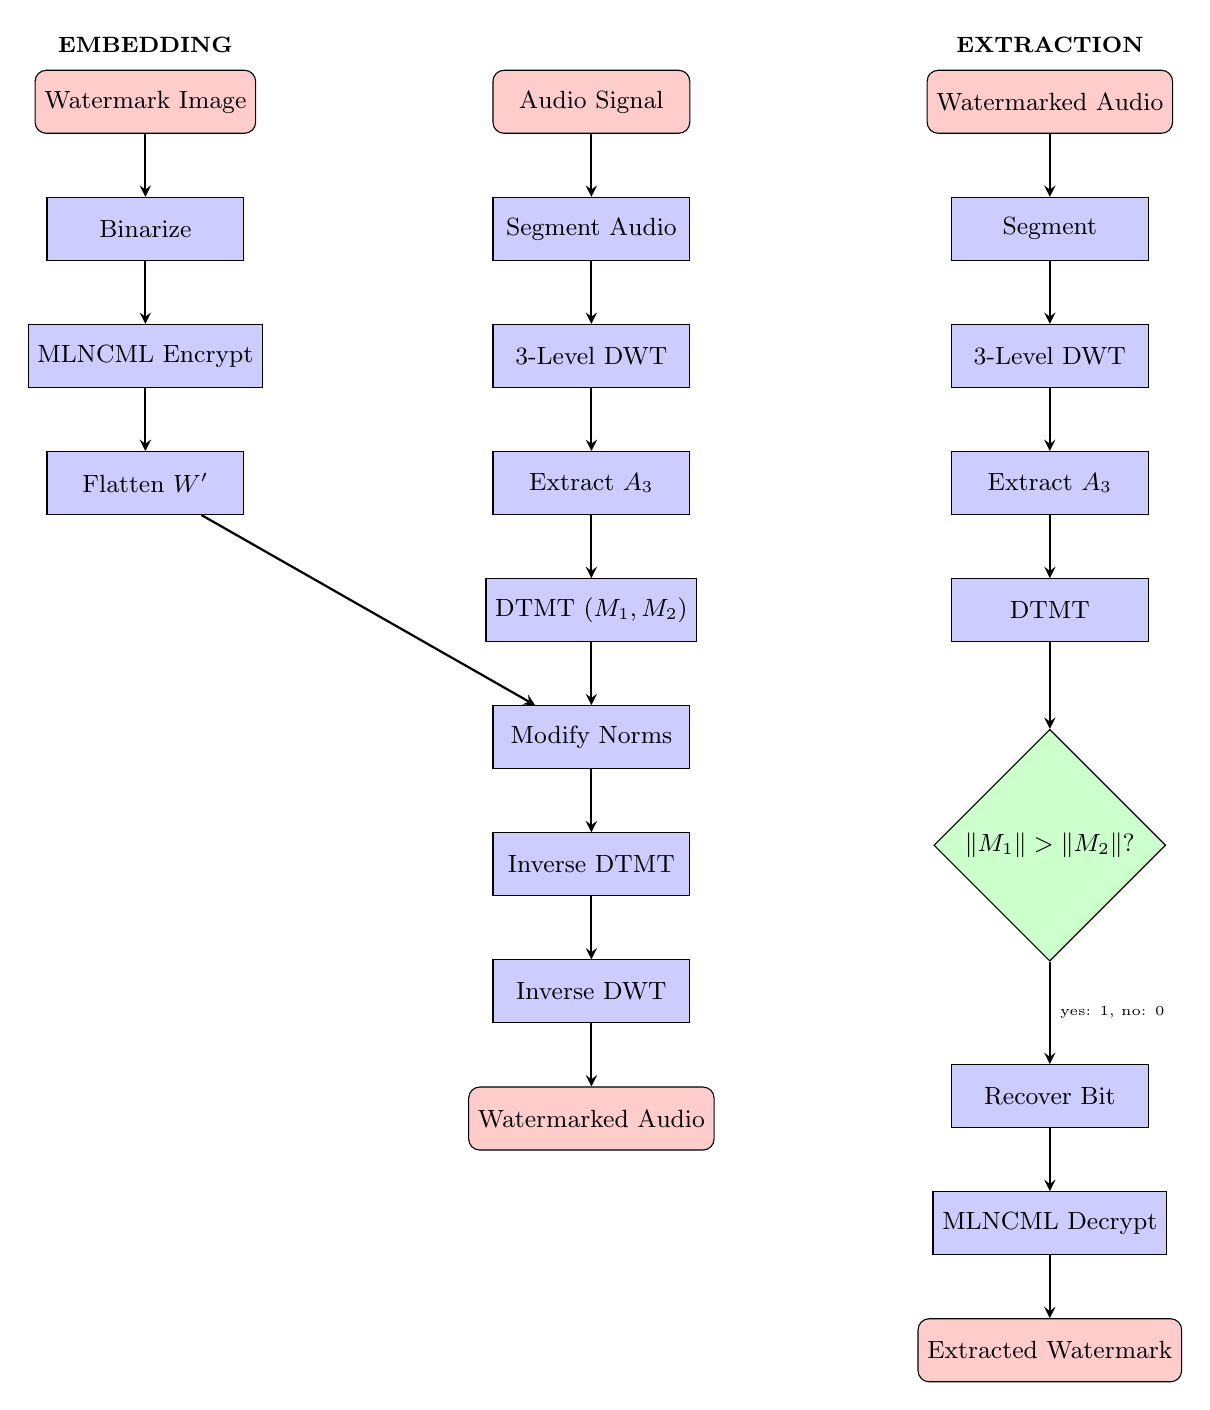
\begin{tikzpicture}[
    node distance=0.8cm and 1.2cm,
    startstop/.style={rectangle, rounded corners, minimum width=2.5cm, minimum height=0.8cm, text centered, draw=black, fill=red!20, font=\small},
    process/.style={rectangle, minimum width=2.5cm, minimum height=0.8cm, text centered, draw=black, fill=blue!20, font=\small},
    decision/.style={diamond, minimum width=2cm, minimum height=0.8cm, text centered, draw=black, fill=green!20, font=\small},
    arrow/.style={thick,->,>=stealth}
    ]
    
    % Embedding path
    \node (img) [startstop] {Watermark Image};
    \node (binarize) [process, below=of img] {Binarize};
    \node (mlncml) [process, below=of binarize] {MLNCML Encrypt};
    \node (flatten) [process, below=of mlncml] {Flatten $W'$};
    
    \node (audio) [startstop, right=3cm of img] {Audio Signal};
    \node (segment) [process, below=of audio] {Segment Audio};
    \node (dwt) [process, below=of segment] {3-Level DWT};
    \node (extract) [process, below=of dwt] {Extract $A_3$};
    \node (dtmt) [process, below=of extract] {DTMT ($M_1, M_2$)};
    \node (modify) [process, below=of dtmt] {Modify Norms};
    \node (idtmt) [process, below=of modify] {Inverse DTMT};
    \node (idwt) [process, below=of idtmt] {Inverse DWT};
    \node (watermarked) [startstop, below=of idwt] {Watermarked Audio};
    
    % Extraction path
    \node (wm_audio) [startstop, right=3cm of audio] {Watermarked Audio};
    \node (seg2) [process, below=of wm_audio] {Segment};
    \node (dwt2) [process, below=of seg2] {3-Level DWT};
    \node (a3_2) [process, below=of dwt2] {Extract $A_3$};
    \node (dtmt2) [process, below=of a3_2] {DTMT};
    \node (compare) [decision, below=of dtmt2, yshift=-0.3cm] {$\|M_1\| > \|M_2\|$?};
    \node (bit) [process, below=of compare, yshift=-0.5cm] {Recover Bit};
    \node (decrypt) [process, below=of bit] {MLNCML Decrypt};
    \node (extracted) [startstop, below=of decrypt] {Extracted Watermark};
    
    % Arrows - Embedding
    \draw [arrow] (img) -- (binarize);
    \draw [arrow] (binarize) -- (mlncml);
    \draw [arrow] (mlncml) -- (flatten);
    \draw [arrow] (audio) -- (segment);
    \draw [arrow] (segment) -- (dwt);
    \draw [arrow] (dwt) -- (extract);
    \draw [arrow] (extract) -- (dtmt);
    \draw [arrow] (flatten) -- (modify);
    \draw [arrow] (dtmt) -- (modify);
    \draw [arrow] (modify) -- (idtmt);
    \draw [arrow] (idtmt) -- (idwt);
    \draw [arrow] (idwt) -- (watermarked);
    
    % Arrows - Extraction
    \draw [arrow] (wm_audio) -- (seg2);
    \draw [arrow] (seg2) -- (dwt2);
    \draw [arrow] (dwt2) -- (a3_2);
    \draw [arrow] (a3_2) -- (dtmt2);
    \draw [arrow] (dtmt2) -- (compare);
    \draw [arrow] (compare) -- node[right, font=\tiny] {yes: 1, no: 0} (bit);
    \draw [arrow] (bit) -- (decrypt);
    \draw [arrow] (decrypt) -- (extracted);
    
    % Labels
    \node[above=0.1cm of img, font=\footnotesize\bfseries] {EMBEDDING};
    \node[above=0.1cm of wm_audio, font=\footnotesize\bfseries] {EXTRACTION};
    
\end{tikzpicture}
\caption{Watermarking system flowchart showing embedding (left/center) and extraction (right) pipelines}
\label{fig:flowchart}
\end{figure}

\section{Implementation Details}

\subsection{MLNCML Encryption}

The watermark image is binarized and encrypted using MLNCML chaotic maps with key parameters $\epsilon=0.3, \mu=3.99, x_0=0.3456789$. The encrypted watermark $W' = W \oplus H_b$ provides security through chaotic keyspace ($>2^{100}$).

\subsection{Transform Domain Embedding}

We segment the audio into $L_{\text{seg}} = \lceil N \cdot M / L_1 \rceil$ blocks and apply 3-level Haar DWT to extract low-frequency approximation coefficients $A_3$. The $A_3$ band is divided into $L_1=4$ sub-blocks, each transformed using DTMT with Tchebichef polynomials ($K=\min(64, L_2/2)$ orders).

For embedding, we split DTMT moments into even ($M_1$) and odd ($M_2$) indices and modify their norms based on the watermark bit:
\begin{equation}
(\sigma_1', \sigma_2') = 
\begin{cases}
(\bar{\sigma} + \delta, \bar{\sigma} - \delta) & \text{if } b = 1 \\
(\bar{\sigma} - \delta, \bar{\sigma} + \delta) & \text{if } b = 0
\end{cases}
\end{equation}
where $\bar{\sigma} = (\|M_1\| + \|M_2\|)/2$ and $\delta=0.05$ controls embedding strength.

\subsection{Extraction}

The extraction process reverses embedding: we segment the watermarked audio, apply DWT/DTMT, and recover each bit by comparing $\|M_1\|$ vs $\|M_2\|$. The encrypted watermark is then decrypted using the same chaotic key.

\section{Key Implementation Challenges}

\subsection{Transform Selection and Audio Quality}

Embedding in the $A_3$ (low-frequency) band rather than detail bands ($D_1, D_2, D_3$) avoids audible ``tinny'' artifacts. However, some perceptual distortion remains, likely due to:
\begin{itemize}
    \item Hard segmentation boundaries without windowing/overlap
    \item Inverse DTMT approximation error from truncated Tchebichef orders
    \item Insufficient normalization after reconstruction
\end{itemize}

\subsection{Parameter Tuning}

The embedding strength $\delta=0.05$ balances imperceptibility and robustness. The DTMT order $K = \min(64, L_2/2)$ prevents numerical instability while maintaining embedding capacity. Segmentation with $L_1=4$ sub-blocks per segment provides sufficient capacity for a $32 \times 32$ watermark without excessive fragmentation.

\subsection{Numerical Precision}

Chaotic systems are sensitive to floating-point errors. We ensure consistent encryption/decryption by using fixed key parameters. The Haar DWT is orthogonal but requires careful padding for odd-length signals. DTMT pseudo-inverse ($T^T M'$) introduces slight approximation errors that accumulate across segments.

\section{Experimental Results}

\subsection{Attack Robustness}

We evaluate robustness on ``The\_Color\_Violet.wav'' with a $32 \times 32$ watermark against four DSP attacks. Metrics: \textbf{SNR} (signal quality, higher better), \textbf{BER} (bit error rate, lower better), \textbf{NC} (normalized correlation, closer to 1 better).

\begin{table}[h]
\centering
\caption{Watermark robustness under DSP attacks}
\label{tab:results}
\begin{tabular}{@{}lccc@{}}
\toprule
\textbf{Attack} & \textbf{SNR (dB)} & \textbf{BER} & \textbf{NC} \\
\midrule
LPF 4000 Hz     & --- & --- & --- \\
HPF 300 Hz      & --- & --- & --- \\
CROP 20\%       & --- & --- & --- \\
Gaussian 20 dB  & --- & --- & --- \\
\bottomrule
\end{tabular}
\end{table}

\textit{Fill values from \texttt{results/attack\_results/results\_summary.csv} after running \texttt{test\_main.py}.}

\section{Conclusion}

We successfully implemented a blind audio watermarking system combining DWT, DTMT, and MLNCML in Python. The system achieves secure embedding through chaotic encryption and reasonable imperceptibility under normal listening conditions. Key learnings include the tradeoff between robustness and audio quality when choosing transform bands, the importance of numerical precision in chaotic systems, and the impact of segmentation strategies on perceptual quality.

\textbf{Future work:} Adaptive embedding strength using psychoacoustic masking, error correction coding for improved BER, overlapping segments with windowing to reduce boundary artifacts, and alternative wavelet families (Daubechies, Symlet) for better frequency localization.

\end{document}

